% Intended LaTeX compiler: pdflatex
\documentclass[a4j, 11pt]{jarticle}
\usepackage[dvipdfmx]{graphicx}
\usepackage[dvipdfmx]{color}
\usepackage{indentfirst}
\usepackage{fancyhdr}
\usepackage{lastpage}
\usepackage{amsmath, amssymb, bm}
\usepackage{minted}
\makeatletter
\author{201611350 江畑 拓哉}
\date{2017年10月19日}
\title{演習課題3}

\pagestyle{fancy}

% headers & footers
\lhead{数理アルゴリズム \@title 提出日:\@date\\\@author}
\chead{}
\rhead{}
\lfoot{}
\cfoot{\thepage /\pageref{LastPage}}
\rfoot{}
\renewcommand{\headrulewidth}{0pt}
\renewcommand{\footrulewidth}{0pt}
\makeatother

\begin{document}

\section{課題1}
\label{sec:org4f62ef8}
ガウス・ザイデル法によって求めるプログラムを次に示す手順に従って作成せよ。\\
\subsection{\(n = 5\) とし、初期値を \(u_{i, j} = 0(1 \leq i, j \leq n)\) とした、ガウス・ザイデル法の反復1ステップ飲みのプログラムを以下に示す。プログラム内の空欄 (a), (b), (c) に入るコードを示せ。}
\label{sec:org2f627ef}
\begin{minted}[frame=lines,linenos=true,obeytabs,tabsize=4]{scilab}
n = 5;
u = zeros(n+2, n+2); // initialize
u(:, n+2) = 100;     // settings for boundary condition
for i = 2:n+1,
    for j = 2:n+1,
        r = 1/4 * (u(i+1, j) + u(i-1, j) + u(i, j+1) + u(i, j-1)) - u(i, j);
        u(i, j) = u(i, j) + r;
    end
end
\end{minted}
\subsection{\(R\leq 10^-2\) となるまで反復計算を行い、反復終了時の \(u_{i, j}\) の値を求めよ。}
\label{sec:org259d515}
\begin{eqnarray*}
R = \max_{1 \leq i, j \leq n} |r_{i, j}|
\end{eqnarray*}
 以下が一回の反復計算で更新される R を得る関数である。\\
\begin{minted}[frame=lines,linenos=true,obeytabs,tabsize=4]{scilab}
function [u, R] = get_R(u, n)
r = ones(n+2, n+2)
for i = 2:n+1,
  for j = 2:n+1,
    r(i, j) = 1/4 * (u(i+1, j) + u(i-1, j) + u(i, j+1) + u(i, j-1)) - u(i, j);
    u(i, j) = u(i, j) + r(i, j);
  end
end
R = max(abs(r(2:n+1,2:n+1)))
endfunction
\end{minted}
 これを R が条件を満たすまで繰り返せば良い。\\
\begin{minted}[frame=lines,linenos=true,obeytabs,tabsize=4]{scilab}
n = 5;
u = zeros(n+2, n+2);
u(:, n+2) = 100;
R = 100;
while R > 10^-2,
  [u, R] = get_R(u, n);
end
u
\end{minted}

 出力\\
\begin{eqnarray*}
\left(   \begin{array}{lllllll}
0. & 0.        & 0.        & 0.        & 0.        & 0.        & 100. \\
0. & 3.1207452 & 7.1626639 & 13.445686 & 24.540364 & 46.862742 & 100. \\
0. & 5.3308847 & 12.097434 & 22.091606 & 37.860954 & 62.913577 & 100. \\
0. & 6.1185691 & 13.820433 & 24.976222 & 41.907186 & 66.933585 & 100. \\
0. & 5.3348475 & 12.103378 & 22.097551 & 37.865431 & 62.915807 & 100. \\
0. & 3.1253686 & 7.1695991 & 13.452622 & 24.545566 & 46.865343 & 100. \\
0. & 0.        & 0.        & 0.        & 0.        & 0.        & 100. \\
\end{array} \right)    
\end{eqnarray*}
\subsection{\(n = 50\) として,ガウス・ザイデル法を実行せよ.}
\label{sec:org5448c5f}
反復は \(R \leq 10^−3\) となったところで停止せよ.\\
 このときの反復ごとの R の値をグラフに示せ.\\
Rの値に対する片対数グラフを採用した。\\
\begin{minted}[frame=lines,linenos=true,obeytabs,tabsize=4]{scilab}
n = 50;
u = zeros(n+2, n+2);
u(:, n+2) = 100;
R = 100;
s = 1;
R_ = zeros(1, 1000);
while R > 10^-3,
  [u, R] = get_R(u, n);
  R_(1, s) = R;
  s = s+1;
end
plot2d('nl', R_)
\end{minted}

\begin{figure}[htbp]
\centering
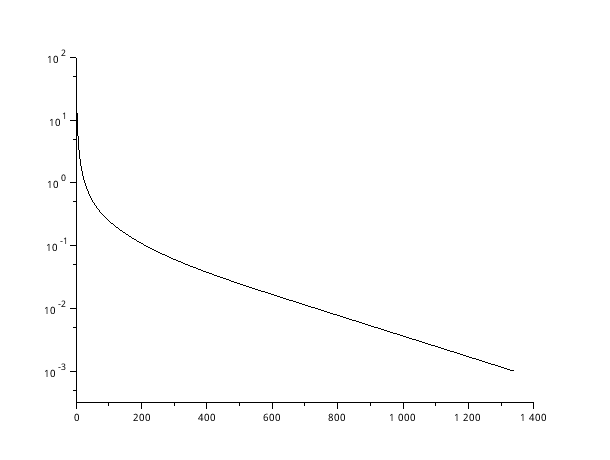
\includegraphics[width=10cm]{./1-3.png}
\caption{Rの値のグラフ}
\end{figure}
\subsection{(1-3) の反復終了時の \(u_{i,j} (0 \leq i, j \leq n + 1)\) の値を Scilab の surf 関数を用いてグラフに描け.}
\label{sec:org90447c0}
surf の使用方法は各自で調べること.\\
\begin{minted}[frame=lines,linenos=true,obeytabs,tabsize=4]{scilab}
surf(linspace(0, 1, 52), linspace(0, 1, 52), u')
\end{minted}
\begin{figure}[htbp]
\centering
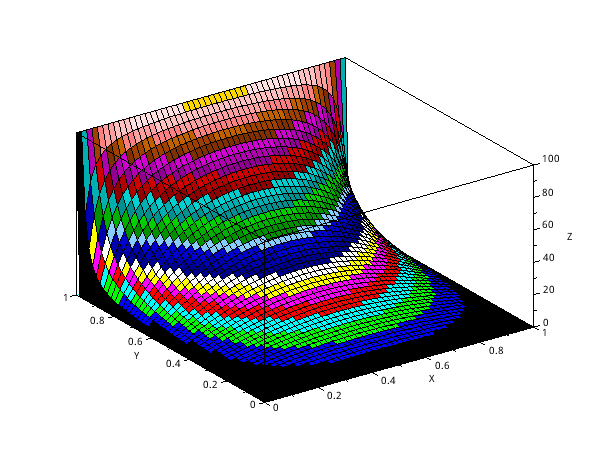
\includegraphics[width=10cm]{./1-4.png}
\caption{u の値のグラフ}
\end{figure}
\section{課題2}
\label{sec:org4ad8538}
\subsection{}
\label{sec:org7461945}
領域 Ω を \([0, 1] \times [0, 1]\) の正方形とし,その境界を Γ とする.関数 \(u(x, y)\) は領域 Ω上で\\
\begin{eqnarray*}
u_{xx} + u_{yy} = 0
\end{eqnarray*}
を満たし,境界 Γ 上での境界条件を以下の式とする.\\
\begin{eqnarray*}
u(x, 0) = sin(\pi x), u(x, 1) = 0 (0 \leq x \leq 1) \\
u(0, y) = 0, u(1, y) = sin(\pi y) (0 \leq y \leq 1)
\end{eqnarray*}
 これらの条件を満たす解 \(u_{i,j} (0 \leq i, j \leq n + 1)\) をガウス・ザイデル法を実行して計算し,反復終了時の \(u_{i,j}\) の値を Scilab の surf 関数を用いてグラフに描画せよ.\\

\begin{minted}[frame=lines,linenos=true,obeytabs,tabsize=4]{scilab}
n = 50;
x = sin(linspace(0, 1, n+2) * %pi);
u = zeros(n+2, n+2);
u(:, 1) = x;
u(:, 52) = 0;
u(1, :) = 0;
u(52, :) = x;
R = 100
while R > 10^-3,
  [u, R] = get_R(u, n);
end
surf(linspace(0, 1, 52), linspace(0, 1, 52), u')   
\end{minted}
\begin{figure}[htbp]
\centering
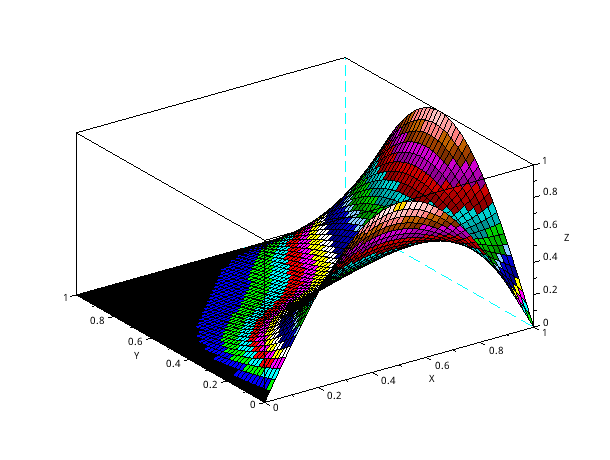
\includegraphics[width=10cm]{./2-1.png}
\caption{u の値のグラフ}
\end{figure}
\subsection{}
\label{sec:orgcde8670}
関数 \(u(x, y)\) は領域 Ω上で\\
\begin{eqnarray*}
u_{xx} + u_{yy} = 0
\end{eqnarray*}
  を満たす。また、外側の正方形の境界を \(\Gamma_1\) ,中央の正方形の境界を \(\Gamma_2\) とする.こ\\
の時,境界 \(\Gamma_1\) , \(\Gamma_2\) で満たすべき条件は\\
\begin{eqnarray*}
u(x, 0) = 0,\ u(x, 1) = 50(1 − x)^4 ,\ u(0, y) = 50y,\ u(1, y) = 0, \\
u(x, 1/3) = u \ u(x, 2/3) = u(1/3, y) = u(2/3, y) = 40\ 
\end{eqnarray*}
となる.これらの条件を満たす解 \(u_{i,j} (0 \leq i, j \leq n + 1)\) をガウス・ザイデル法を用いて計算し,反復終了時の \(u_{i,j}\) の値を surf を用いてグラフに描画せよ.\\
\#+LATEX \newline\\
 以下がこの場合におけるRを得る関数である。\\
\begin{minted}[frame=lines,linenos=true,obeytabs,tabsize=4]{scilab}
function [u, R] = get_R_2(u, n, th1, th2)
r = zeros(n+2, n+2)
for i = 2:n,
  if th1 < i & th1 < th2 then continue end,
  for j = 2:n,
    if th1 < j & j < th2 then continue end, 
    r(i, j) = 1/4 * (u(i+1, j) + u(i-1, j) + u(i, j+1) + u(i, j-1)) - u(i, j);
    u(i, j) = u(i, j) + r(i, j);
  end
end
R = max(abs(r(2:n+1,2:n+1)))
endfunction
\end{minted}
 これを用いてガウス・ザイデル法を適用する。\\
\begin{minted}[frame=lines,linenos=true,obeytabs,tabsize=4]{scilab}
n = 50;
u = zeros(n+2, n+2);
u(:, 1) = 0;
u(:, 52) = 50 * (1 - linspace(0, 1, 52))^4;
u(1, :) = 50 * linspace(0, 1, 52);
u(52, :) = 0;
u(18:36, 18:36) = 40;
R = 100
s = 1
while R > 10^-3,
  s = s + 1
  [u, R] = get_R_2(u, n, 18, 36);
end
s
u(18:36, 18:36) = 0;
surf(linspace(0, 1, 52), linspace(0, 1, 52), u')   
\end{minted}
\begin{figure}[htbp]
\centering
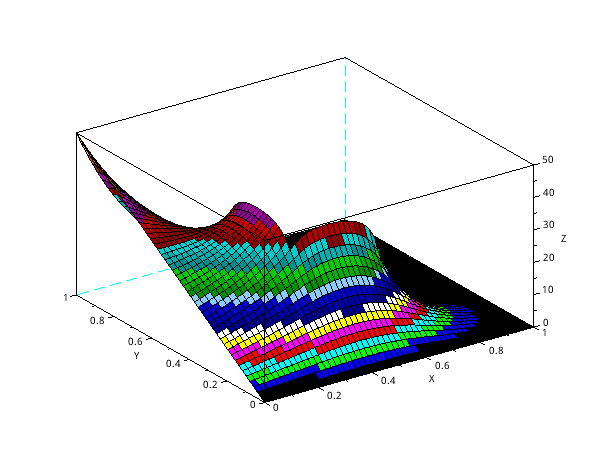
\includegraphics[width=10cm]{./2-2.png}
\caption{u の値のグラフ}
\end{figure}
\end{document}
